\documentclass{article}
\usepackage[utf8]{inputenc}

\title{\textbf{Project Assignment \#1} \\ Robby the Soda Can Collector}
\author{Kerem Bozdaş}
\date{March 2014}

\usepackage{natbib}
\usepackage{graphicx}
\usepackage{color}

\begin{document}

\maketitle

\section{Plot of Fitness Scores}
The plot for the best performing robots (with default parameters) could be seen below in Figure \ref{fig:fitness}.

\begin{figure}[h!]
\centering
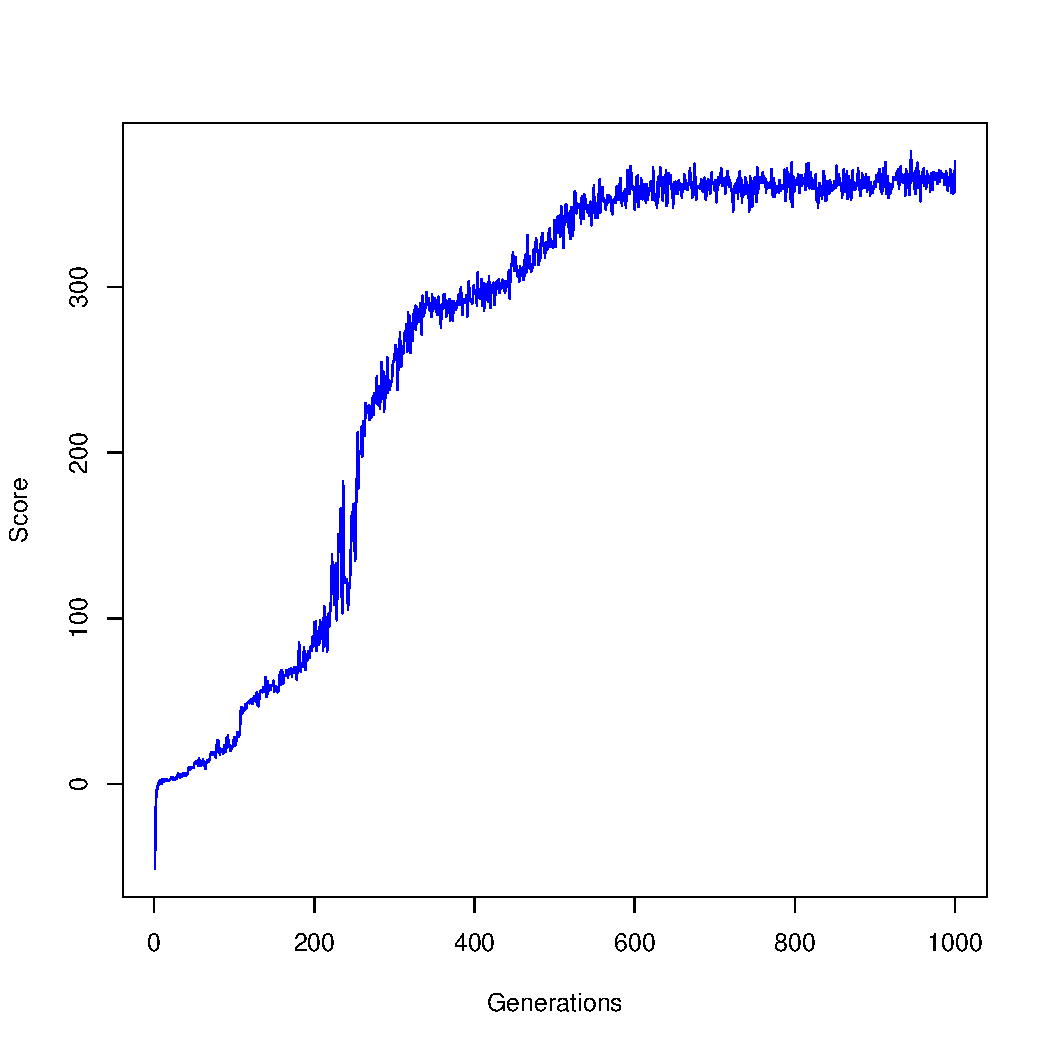
\includegraphics[scale=0.56]{figure-1.pdf}
\caption{Best performing robots through generations}
\label{fig:fitness}
\end{figure}


\section{Changes in Mutation Probability}
We observe the score stalling after a short period of time in in Figure \ref{fig:fitness-no-mutation} when mutation probability is set to zero.

\begin{figure}[h!]
\centering
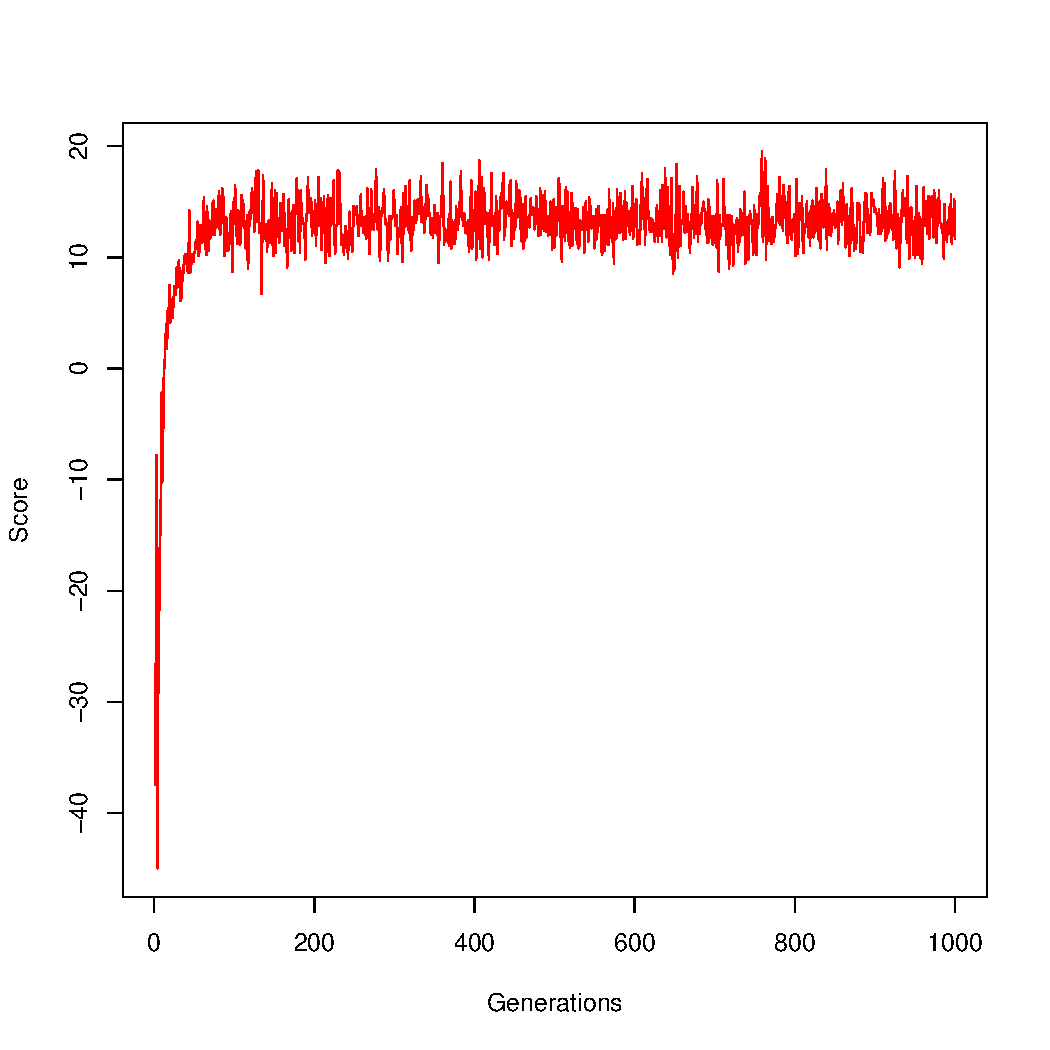
\includegraphics[scale=0.56]{figure-2.pdf}
\caption{Best performing robots through generations (no mutation)}
\label{fig:fitness-no-mutation}
\end{figure}

\clearpage

\subsection{Discussion}
If we compare previous figures, we can see that the robots with zero mutation probability score poorly in their following generations. The comparison could be seen in Figure \ref{fig:fitness-comparison}.

\begin{figure}[h!]
\centering
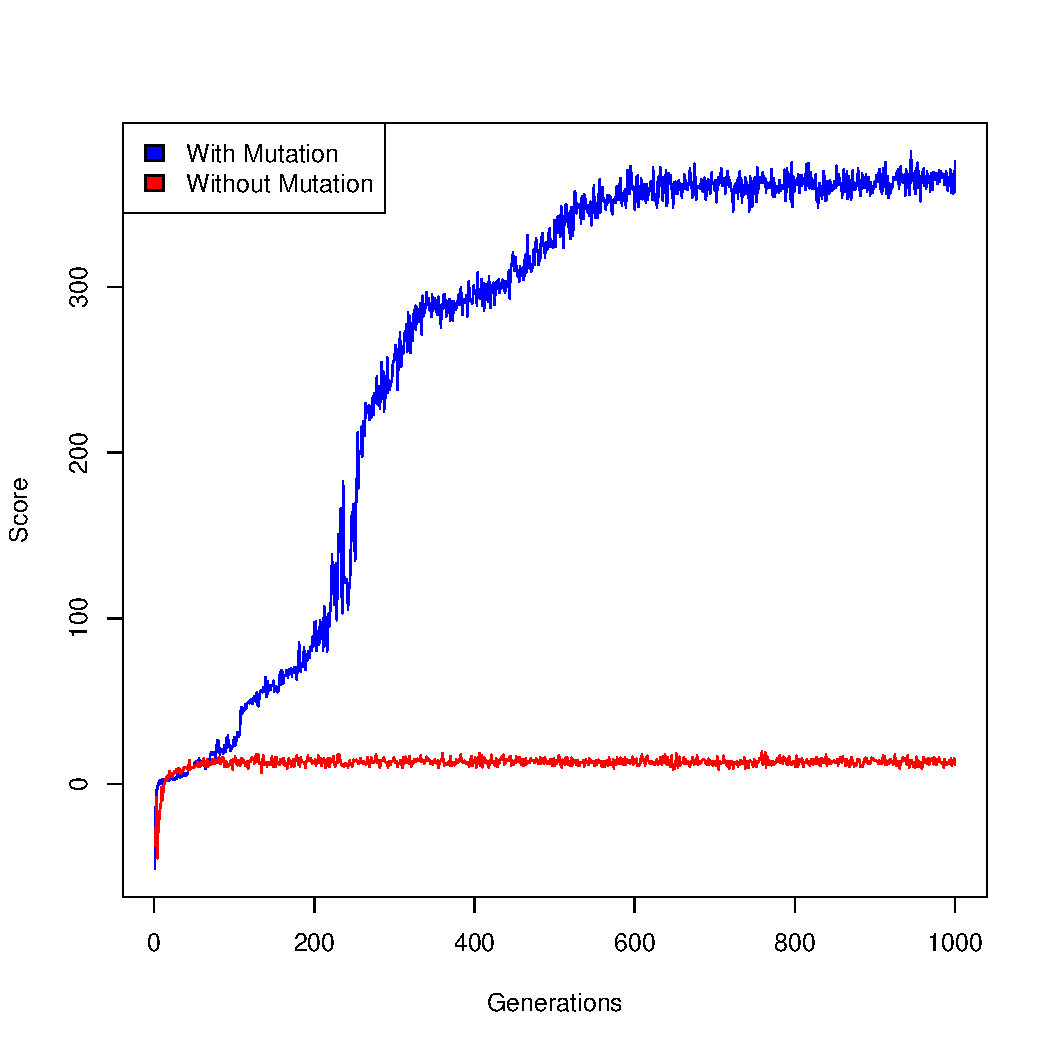
\includegraphics[scale=0.56]{figure-3.pdf}
\caption{Comparison of generations in contrast of mutation probabilities}
\label{fig:fitness-comparison}
\end{figure}

\clearpage

\section{Indexing}
``I always thought something was fundamentally wrong with the universe'' \citep{adams1995hitchhiker}

\definecolor{light-gray}{gray}{0.70}
\definecolor{darkish-gray}{gray}{0.45}

\textcolor{light-gray}{(This is a part in progress.)}


\section{STAY\_PUT Actions}
The average usage of the STAY\_PUT operation for a generation (calculated among 1000 generations) is $50.88$, and for a single robot: $0.2544$. The standard deviation for the number of STAY\_PUT actions is $11.48676$. We can observe decrease in the amount of STAY\_PUT actions through generations as our robot gets clever (or rather, less stupid). The plot for this could be seen below in Figure 4.

\begin{figure}[h!]
\centering
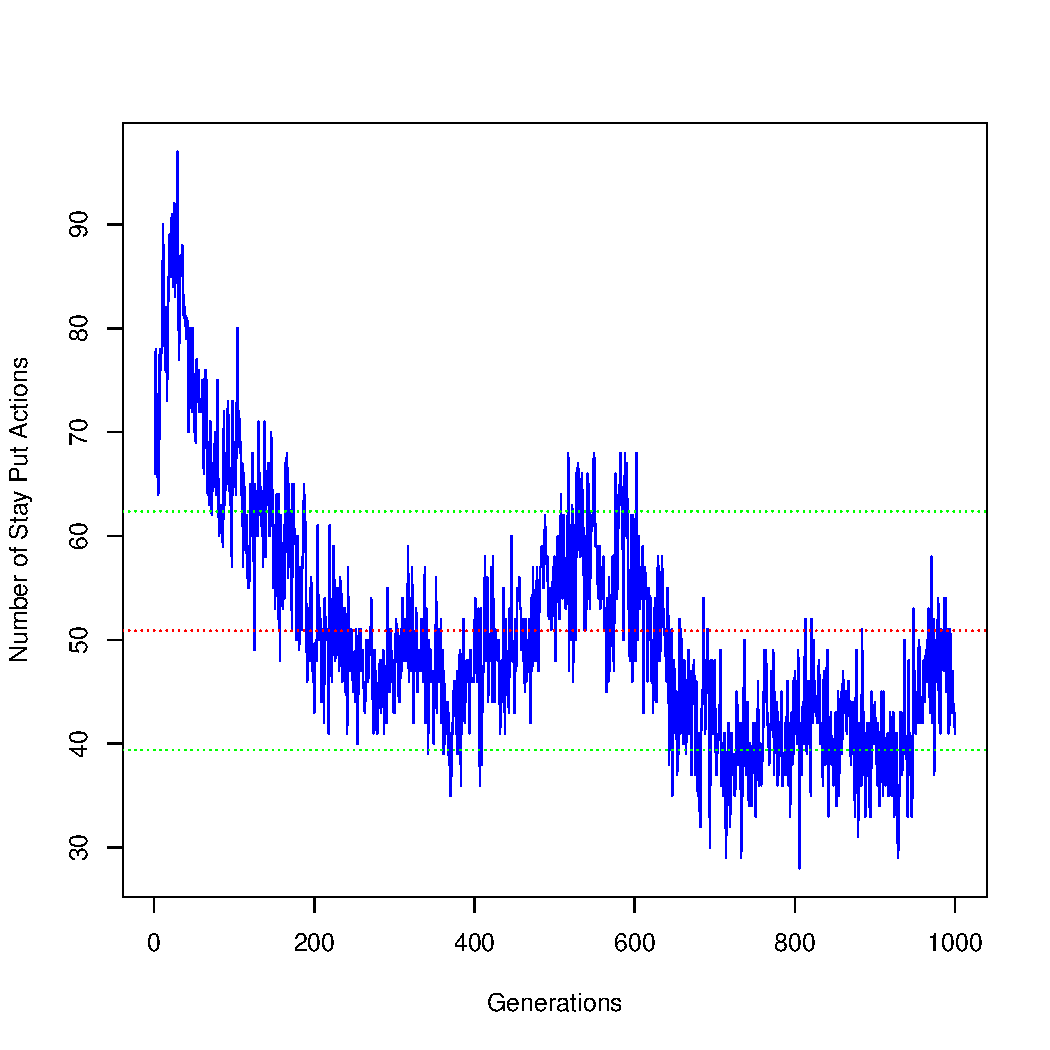
\includegraphics[scale=0.56]{figure-4.pdf}
\caption{The decrease in STAY\_PUT actions as generation id increases}
\label{fig:stay-put-actions}
\end{figure}


\bibliographystyle{plain}
\bibliography{references}
\end{document}
